\documentclass[a4paper,9pt]{beamer}\usepackage[]{graphicx}\usepackage[]{color}
%% maxwidth is the original width if it is less than linewidth
%% otherwise use linewidth (to make sure the graphics do not exceed the margin)
\makeatletter
\def\maxwidth{ %
  \ifdim\Gin@nat@width>\linewidth
    \linewidth
  \else
    \Gin@nat@width
  \fi
}
\makeatother

\definecolor{fgcolor}{rgb}{0.345, 0.345, 0.345}
\newcommand{\hlnum}[1]{\textcolor[rgb]{0.686,0.059,0.569}{#1}}%
\newcommand{\hlstr}[1]{\textcolor[rgb]{0.192,0.494,0.8}{#1}}%
\newcommand{\hlcom}[1]{\textcolor[rgb]{0.678,0.584,0.686}{\textit{#1}}}%
\newcommand{\hlopt}[1]{\textcolor[rgb]{0,0,0}{#1}}%
\newcommand{\hlstd}[1]{\textcolor[rgb]{0.345,0.345,0.345}{#1}}%
\newcommand{\hlkwa}[1]{\textcolor[rgb]{0.161,0.373,0.58}{\textbf{#1}}}%
\newcommand{\hlkwb}[1]{\textcolor[rgb]{0.69,0.353,0.396}{#1}}%
\newcommand{\hlkwc}[1]{\textcolor[rgb]{0.333,0.667,0.333}{#1}}%
\newcommand{\hlkwd}[1]{\textcolor[rgb]{0.737,0.353,0.396}{\textbf{#1}}}%
\let\hlipl\hlkwb

\usepackage{framed}
\makeatletter
\newenvironment{kframe}{%
 \def\at@end@of@kframe{}%
 \ifinner\ifhmode%
  \def\at@end@of@kframe{\end{minipage}}%
  \begin{minipage}{\columnwidth}%
 \fi\fi%
 \def\FrameCommand##1{\hskip\@totalleftmargin \hskip-\fboxsep
 \colorbox{shadecolor}{##1}\hskip-\fboxsep
     % There is no \\@totalrightmargin, so:
     \hskip-\linewidth \hskip-\@totalleftmargin \hskip\columnwidth}%
 \MakeFramed {\advance\hsize-\width
   \@totalleftmargin\z@ \linewidth\hsize
   \@setminipage}}%
 {\par\unskip\endMakeFramed%
 \at@end@of@kframe}
\makeatother

\definecolor{shadecolor}{rgb}{.97, .97, .97}
\definecolor{messagecolor}{rgb}{0, 0, 0}
\definecolor{warningcolor}{rgb}{1, 0, 1}
\definecolor{errorcolor}{rgb}{1, 0, 0}
\newenvironment{knitrout}{}{} % an empty environment to be redefined in TeX

\usepackage{alltt}
\usepackage[]{graphicx}
\usepackage[]{color}
\usepackage{alltt}
\usepackage{amsmath}
\usepackage{amsfonts}
\usepackage{amssymb}
\usepackage{verbatim}
\usepackage{hyperref}

\title{Computer Intensive Methods\\Presentation 1}
\author[Jorriet,Olusoji,Orlowski,Olusoji]{Jorriet Marc\inst{1}{()}, Olusoji Oluwafemi\inst{1}{(1541893)}, \inst{1}Orlowski Robert\inst{1}{(1541889)}, Owokotomo Olajumoke Evangelina\inst{1}{(1539654)}}
\institute[UHasselt]{\inst{1} Center for Statistics and Biostatistics, Universiteit Hasselt, Agoralaan D, 3590, Diepenbeek, Belgium.}
\date{\today}
\IfFileExists{upquote.sty}{\usepackage{upquote}}{}
\begin{document}



\frame[plain]{\maketitle}

\begin{frame}{Table of Contents}
\tableofcontents
\end{frame}

%\section{Question 1}

%\section{Question 2}

\section{Question 3}
\subsection{Nonparametric Bootstrap Approximation}
\begin{frame}{Exploration \& Bootstrap Algorithm (Nonparametric)}
\begin{columns}
\column{0.4\textwidth}
\begin{knitrout}
\definecolor{shadecolor}{rgb}{0.969, 0.969, 0.969}\color{fgcolor}
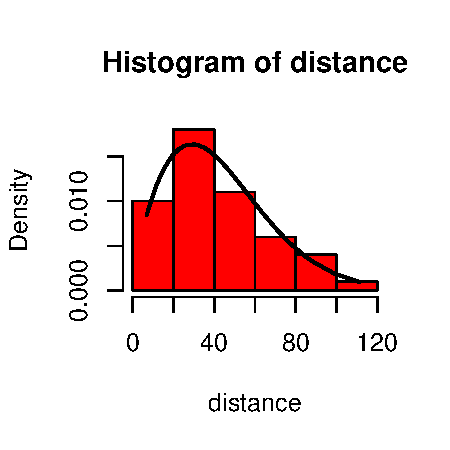
\includegraphics[width=\maxwidth]{figure/explore3-1} 

\end{knitrout}
\column{0.6\textwidth}
\begin{enumerate}[i]
\item Draw $B=5000, 50000, 100000$ from the data (stopping distance) with replacement
\item Compute statistic of interest(maximum) from each bootstrap sample(bootstrap replicates)
\item Approximate $se(\hat{\theta})$ by the sample standard deviation of bootstrap replicates.
\end{enumerate}
\end{columns}
\end{frame}

\begin{frame}{Results, Problem \& Remedies}

% <<,fig.height=2,fig.width=3>>=
% #par(mfrow=c(2,2))
% #for(i in seq_along(results3)){
% hist(results3[[1]],main=paste(boot_length[1],'replicates',sep=' '),xlab=expression(theta^'*'))
% #}
% @

\begin{columns}
\column{0.5\textwidth}
\begin{block}{Results}
\begin{table}[h]
\begin{tabular}{cccc}
\hline
Replicates & 5000 & 50000 & 100000\\ 
\hline
SError & 13.75 & 13.74 & 13.77\\
\hline
\end{tabular}
\caption{Standard Error estimates}
\end{table}
\end{block}
\column{0.5\textwidth}
\begin{block}{Problems and Remedy}
\begin{itemize}
\item Discrete not continuous distribution observed (\alert{see Appendix graph})
\item Poor approximation of the distribution of maximum (\alert{Bickel, Gotze, and van Zwet (1997)}) but standard error still appropriately computed.
\item Remedy includes m out of n bootstrapp (\alert{Bickel, Gotze, and van Zwet (1997)}) and Semiparametric bootstrapp (\alert{Zelterman (1993)}).
\end{itemize}
\end{block}
\end{columns}
\end{frame}

\subsection{Parametric Bootstrap}
\begin{frame}{Bootstrap Algorithm (Parametric)}
\begin{columns}
\column{0.4\textwidth}
Candidate distributions based on extreme value theories include;
\begin{enumerate}[i]
\item Gumbel
\item Weibull
\item Generalized extreme value distribution (GEV)
\end{enumerate}

\column{0.6\textwidth}
\begin{enumerate}[i]
\item Draw $B=5000, 50000, 100000$ from a \alert{distribution that best summarizes(weibull)} the data with parameters replaced with their plugin estimates(1.7239251, 48.1481931)
\item Compute statistic of interest(maximum) from each bootstrap sample(bootstrap replicates)
\item Approximate $se(\hat{\theta})$ by the sample standard deviation of bootstrap replicates.
\end{enumerate}
\end{columns}

\alert{Question of the best distribution to assume}
\begin{table}[h]
\begin{tabular}{cccc}
\hline
& Gumbel & \alert{Weibull} & GEV\\
\hline
AIC & 462.72 & \alert{461.47} & 464.72\\
\hline
\end{tabular}
\caption{AIC values of Candidate distributions}
\end{table}

\end{frame}

\begin{frame}{Results \& Comarison}


\begin{columns}
\column{0.5\textwidth}
\begin{block}{Results}
\begin{table}[h]
\begin{tabular}{cccc}
\hline
Replicates & 5000 & 50000 & 100000\\ 
\hline
SError & 17.9 & 18.25 & 18.24\\
\hline
\end{tabular}
\caption{Standard Error estimates}
\end{table}
\end{block}

\column{0.5\textwidth}
\begin{block}{Comparison \& Discussions}
\begin{enumerate}[i]
\item Continuous and not discrete distribution observed.
\item Standard error computed larger than that of the semi-parametric bootstrapp.
\item This is partly because of the distribution used.
\end{enumerate}
\end{block}
\end{columns}
\end{frame}

\subsection{Probability of High Risk Stopping Distance}
\begin{frame}{Bootstrap Algorithm (Non-Parametric) \& Results}

\begin{columns}
\column{0.5\textwidth}
\begin{block}{Algorithm}
\begin{enumerate}[i]
 \item Draw $B=5000, 50000, 100000$ from the data (stopping distance) with replacement
 \item Compute probability of interest $P(distance > 65ft) = \frac{\#(distance > 65)}{n}$ from each bootstrap sample (bootstrap replicates)
 \item Approximate $P(distance > 65ft)$ by the mean of bootstrap replicates.
 \end{enumerate}
 \end{block}
 
 \column{0.5\textwidth}
 \begin{block}{Results}
 \begin{table}[h]
\begin{tabular}{cccc}
\hline
Replicates & 5000 & 50000 & 100000\\ 
\hline
Prob. & 0.2 & 0.2 & 0.2\\
\hline
\end{tabular}
\caption{Standard Error estimates}
\end{table}

 \end{block}
\end{columns}
\end{frame}


\section{Question 4}
\subsection{Computing Odds Ratio}

\begin{frame}{Odds Ratio and Confidence Interval}
\begin{columns}
\column{0.5\textwidth}
\begin{knitrout}
\definecolor{shadecolor}{rgb}{0.969, 0.969, 0.969}\color{fgcolor}
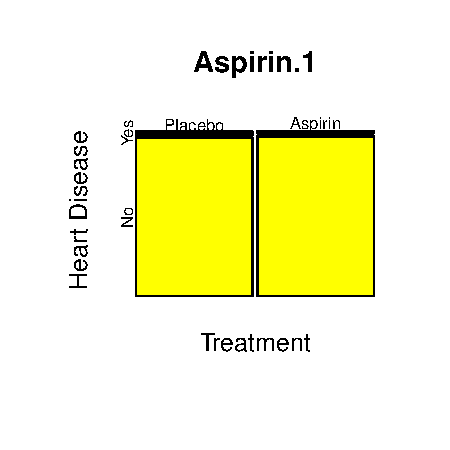
\includegraphics[width=\maxwidth]{figure/oddsplot-1} 

\end{knitrout}
\column{0.5\textwidth}
\begin{block}{Results}
\begin{enumerate}[i]
\item Observation unit are
\item Odds ratio is 1.83(1.44,2.33)
\item The odds of.....
\end{enumerate}
\end{block}
\end{columns}
\end{frame}

\subsection{Bootstrap Approach}


\begin{frame}{Bootstrap Algorithm and Results}
\begin{columns}
\column{0.5\textwidth}
\begin{block}{Bootstrap t Algorithm}
\begin{enumerate}[i]
\item Draw B = 5000 and 50000 bootstrap samples from the data and compute $Z^* = \frac{\hat{\theta^*} - \hat{\theta}}{\hat{se(\theta^*)}}$, where $\hat{\theta^*}$ is the bootstrap log-odds and $\hat{se(\theta^*)}$ is the corresponding bootstrap standard error.
\item \alert{Note that pairs are sampled}
\item obtain quantiles of the replicate $Z^*$
\item Compute $(\hat{\theta} - \hat{t}_{1-\alpha}se(\hat{\theta}),\hat{\theta} + \hat{t}_{\alpha}\hat{se(\theta)})$, where $\hat{\theta}$ is the estimated log odds ratio and $se(\hat{\theta})$ is the estimated standard error of the odds ratio.
\end{enumerate}
\end{block}

\column{0.5\textwidth}
\begin{block}{Results}
\begin{table}[h]
\begin{tabular}{ccc}
\hline
Replicates & 5000 & 50000\\
\hline
Quantiles & \ensuremath{-2.01},1.99 & \ensuremath{-1.97},1.93\\
CI & 1.43,2.34 & 1.44,2.32\\
Coverage & 0.95 & 0.95\\
\hline
\end{tabular}
\caption{Bootstrap Quantiles and Confidence Intervals}
\end{table}
\alert{Note that this version of bootstrap is not transformation invariant. Hence building confidence interval for the log-odds without transforming is a better option.}
\end{block}
\end{columns}
\end{frame}

\begin{frame}{Percental Interval(PI)}

\begin{columns}
\column{0.5\textwidth}
\begin{block}{Percentile Interval Algorithm}
\begin{enumerate}[i]
\item Draw B = 5000 and 50000 bootstrap samples from the data with replacement
\item Compute bootstrap replicates (odds ratio).
\item obtain quantiles of the replicates.
\end{enumerate}

\end{block}

\column{0.5\textwidth}
\begin{block}{Results}
\begin{table}[h]
\begin{tabular}{ccc}
\hline
Replicates & 5000 & 50000\\
\hline
CI & 1.43,2.37 & 1.45,2.34\\
Coverage & 0.95 & 0.95\\
\hline
\end{tabular}
\caption{Confidence Intervals}
\end{table}
\end{block}
\end{columns}
\end{frame}

\section{Appendix}
\begin{frame}{Distribution of Bootstrap Replicates (Non Parametric)}
\begin{knitrout}
\definecolor{shadecolor}{rgb}{0.969, 0.969, 0.969}\color{fgcolor}
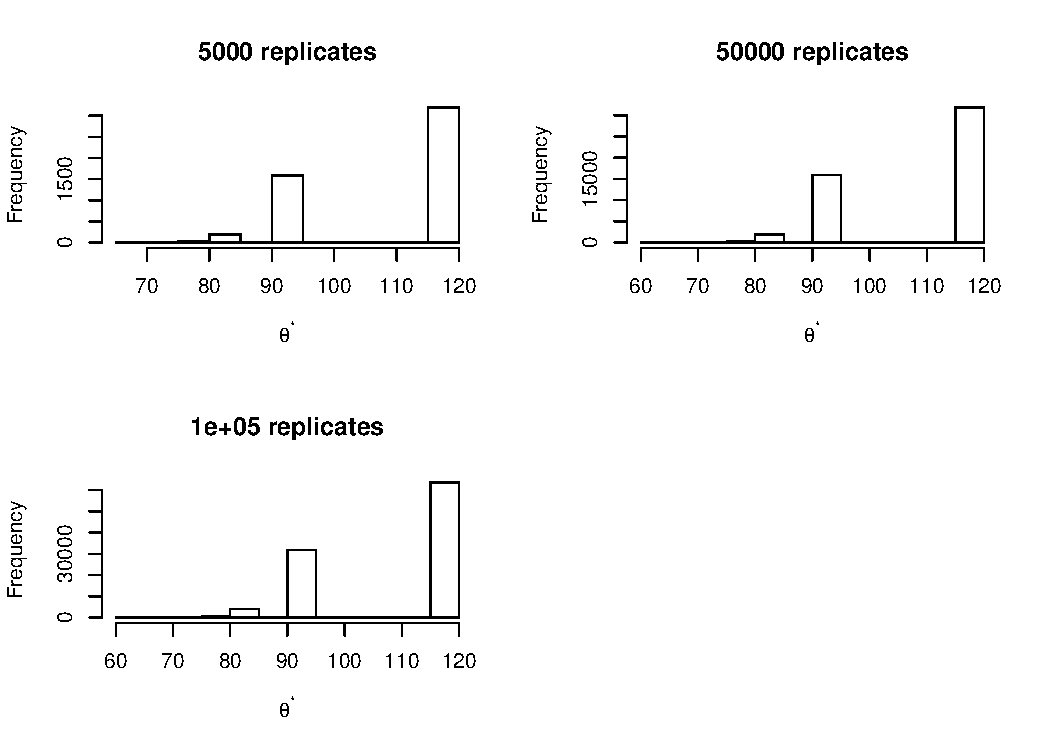
\includegraphics[width=\maxwidth]{figure/plots3-1} 

\end{knitrout}
\end{frame}

\begin{frame}{Distribution of Bootstrap Replicates (Parametric)}
\begin{knitrout}
\definecolor{shadecolor}{rgb}{0.969, 0.969, 0.969}\color{fgcolor}
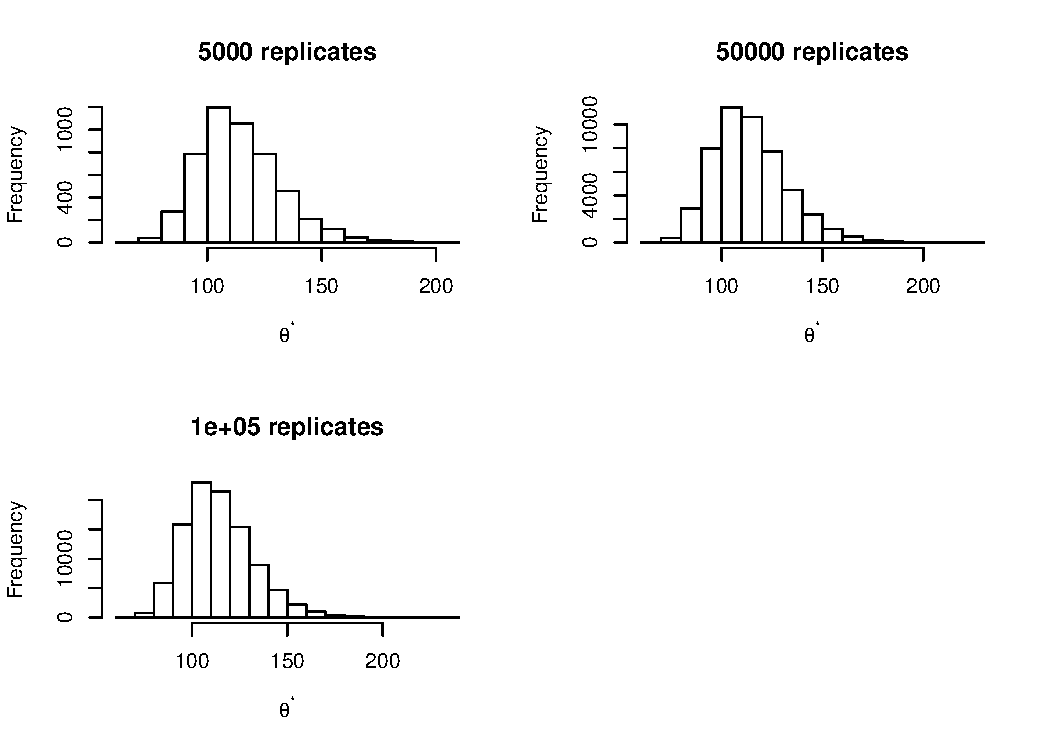
\includegraphics[width=\maxwidth]{figure/plots32-1} 

\end{knitrout}
\end{frame}

\begin{frame}{Distribution of Bootstrap Replicates (Probability)}
\begin{knitrout}
\definecolor{shadecolor}{rgb}{0.969, 0.969, 0.969}\color{fgcolor}
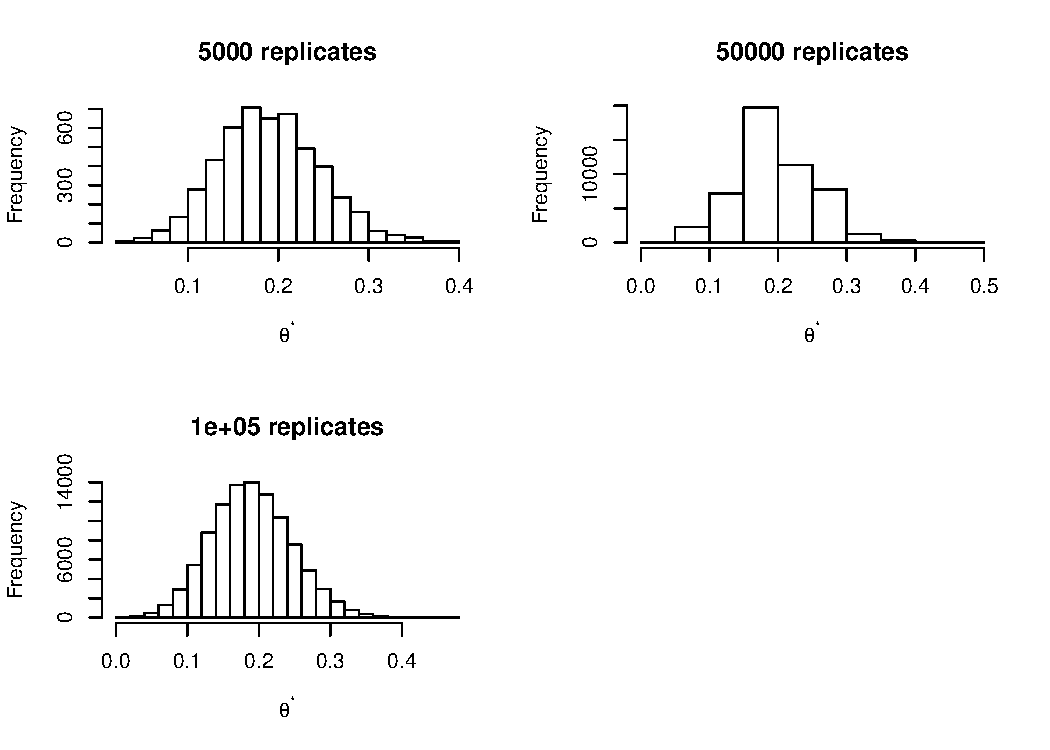
\includegraphics[width=\maxwidth]{figure/plots33-1} 

\end{knitrout}
\end{frame}

\begin{frame}{Distribution of Bootstrap Replicates (Odds Ratio)}
\begin{knitrout}
\definecolor{shadecolor}{rgb}{0.969, 0.969, 0.969}\color{fgcolor}
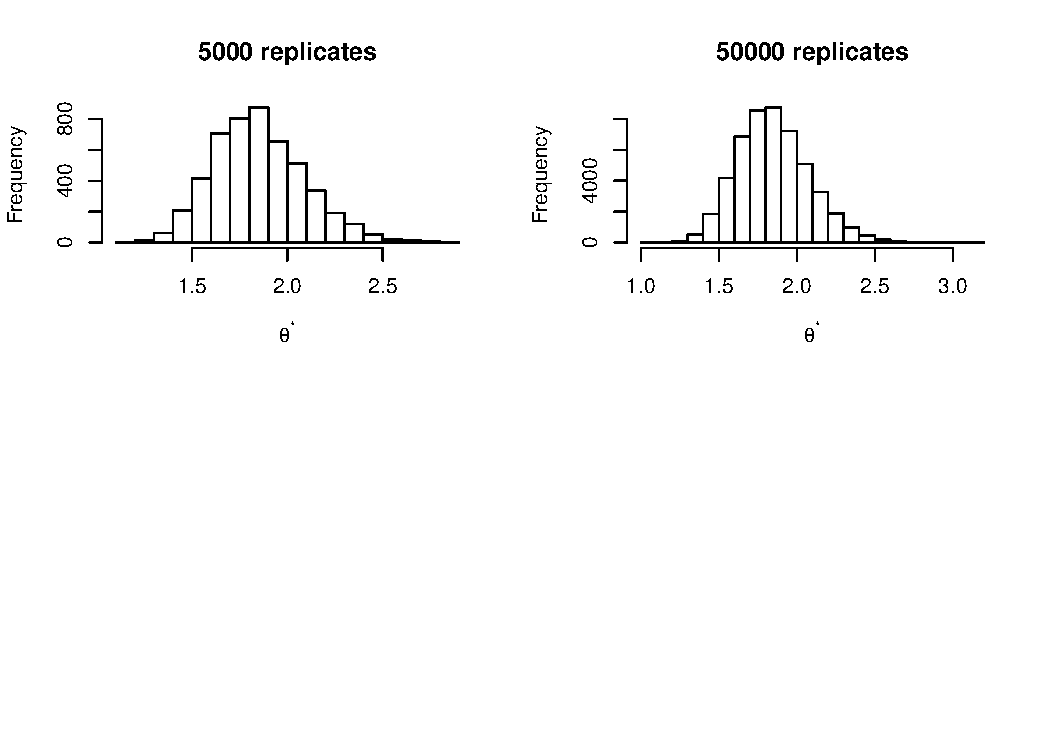
\includegraphics[width=\maxwidth]{figure/plots41-1} 

\end{knitrout}
\end{frame}

\end{document}
